\section{Ewaluacja}
\label{sec:eval}

\subsection{Metryki na walidacji i teście}

Model oceniamy pięcioma metrykami (Tabela~\ref{tab:metrics}). Wszystkie utrzymują się
na poziomie $\sim$0{,}99, co dla tego zbioru oznacza praktyczny sufit jakości.

\begin{table}[H]
  \centering
  \caption{Metryki MLP na zbiorze walidacyjnym i testowym.}
  \label{tab:metrics}
  \begin{tabular}{lcc}
    \toprule
    \textbf{Metryka} & \textbf{Walidacja} & \textbf{Test} \\
    \midrule
    accuracy  & 0{,}9908 & 0{,}9864 \\
    precision & 0{,}9899 & 0{,}9838 \\
    recall    & 0{,}9934 & 0{,}9915 \\
    F1        & 0{,}9916 & 0{,}9877 \\
    ROC-AUC   & 0{,}9992 & 0{,}9987 \\
    \bottomrule
  \end{tabular}
\end{table}

\begin{figure}[H]
  \centering
  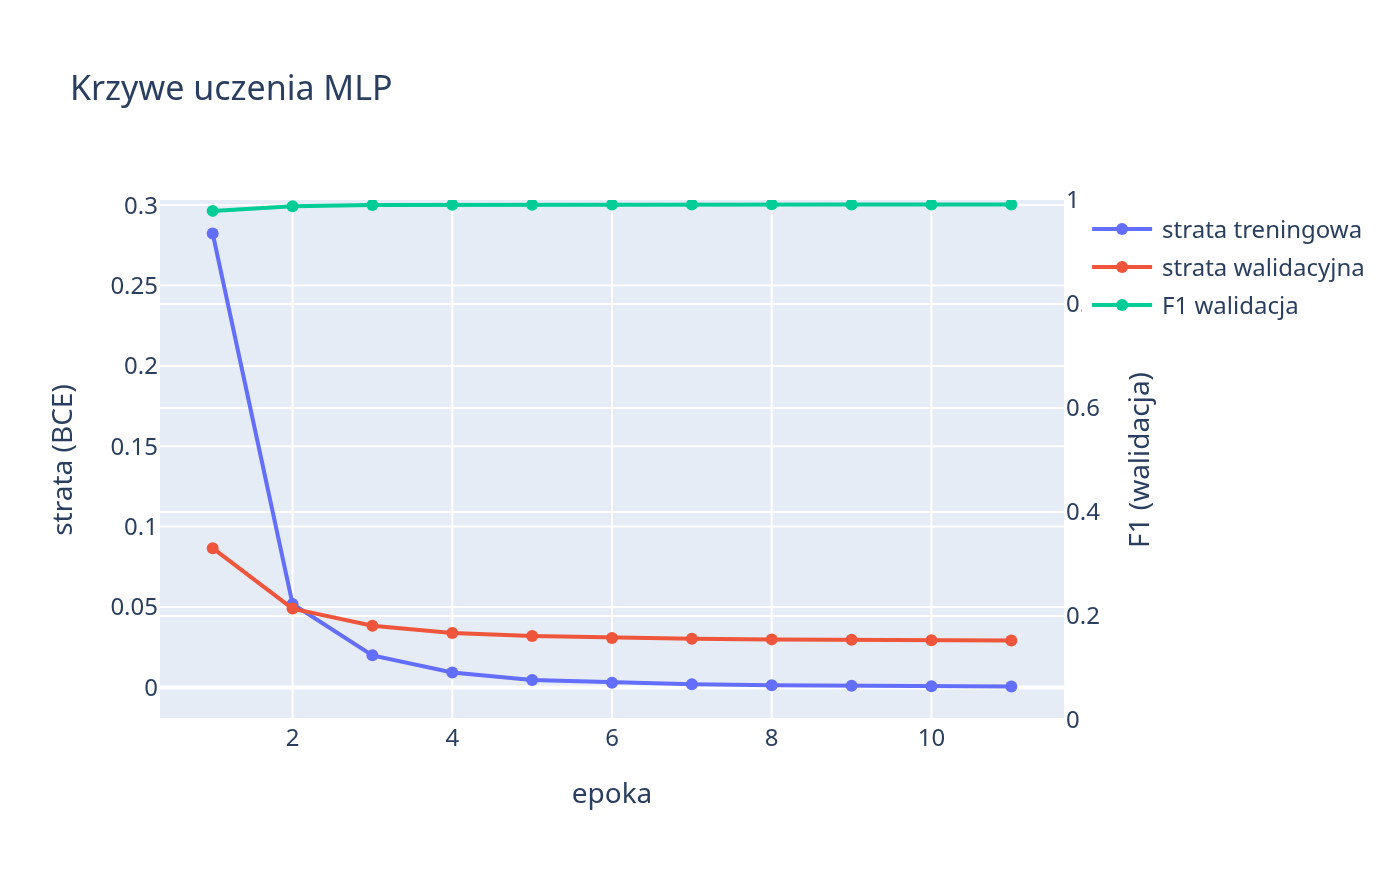
\includegraphics[width=0.78\textwidth]{figures/mlp_krzywe_uczenia.png}
  \caption{Krzywe uczenia MLP: strata treningowa/walidacyjna (oś lewa) oraz F1
  walidacji (oś prawa). Sieć zbiega w pierwszych epokach; early stopping przerywa
  trening, gdy F1 przestaje rosnąć.}
\end{figure}

\begin{figure}[H]
  \centering
  \begin{minipage}{0.48\textwidth}
    \centering
    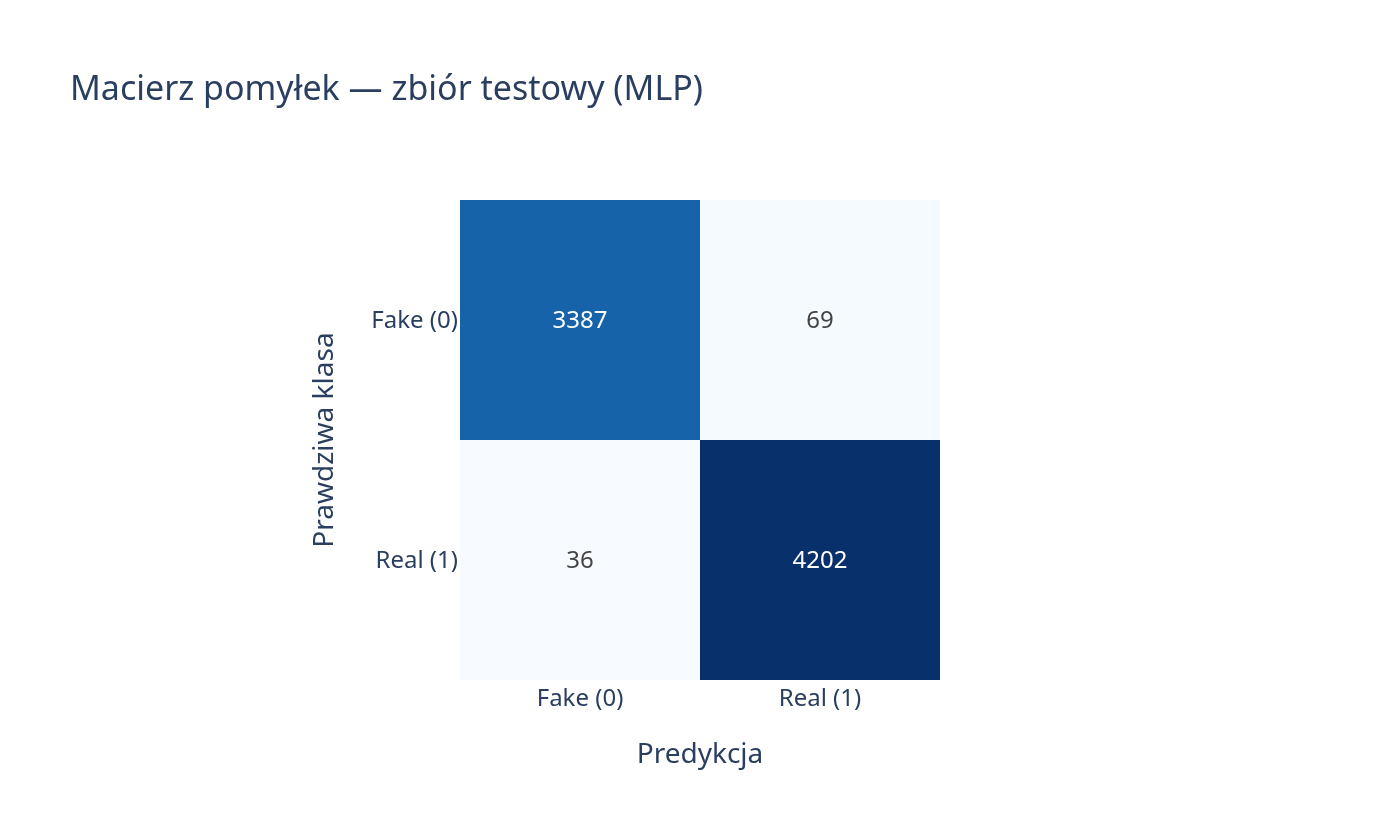
\includegraphics[width=\textwidth]{figures/mlp_macierz_pomylek.png}
  \end{minipage}\hfill
  \begin{minipage}{0.48\textwidth}
    \centering
    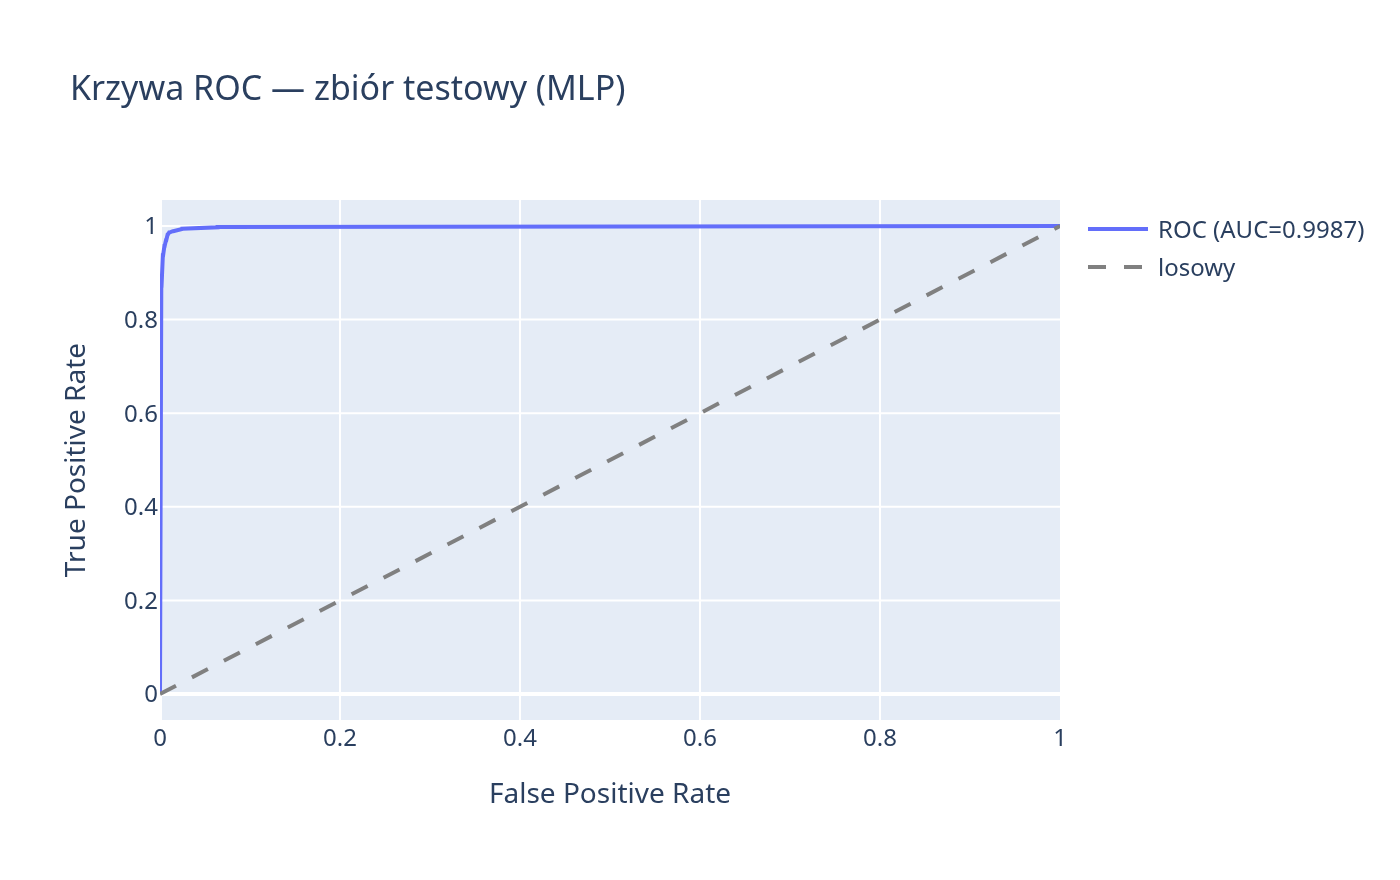
\includegraphics[width=\textwidth]{figures/mlp_roc.png}
  \end{minipage}
  \caption{Macierz pomyłek (po lewej) i krzywa ROC (po prawej) na zbiorze testowym.
  Błędy są nieliczne i rozłożone na obie klasy.}
\end{figure}

\subsection{Porównanie z baselinem (LogReg vs MLP)}

Ponieważ oba modele korzystają z \emph{identycznej} reprezentacji TF-IDF, różnica
wyników izoluje wpływ samej architektury klasyfikatora (Tabela~\ref{tab:compare}).

\begin{table}[H]
  \centering
  \caption{Porównanie na zbiorze testowym.}
  \label{tab:compare}
  \begin{tabular}{lcc}
    \toprule
    \textbf{Metryka} & \textbf{LogReg (baseline)} & \textbf{MLP (od zera)} \\
    \midrule
    accuracy  & 0{,}9795 & \textbf{0{,}9864} \\
    precision & 0{,}9751 & \textbf{0{,}9838} \\
    recall    & 0{,}9880 & \textbf{0{,}9915} \\
    F1        & 0{,}9815 & \textbf{0{,}9877} \\
    ROC-AUC   & 0{,}9970 & \textbf{0{,}9987} \\
    \bottomrule
  \end{tabular}
\end{table}

MLP przewyższa baseline o ok.\ 0{,}6~pp F1 --- różnica marginalna. Na tym leksykalnie
łatwym zbiorze klasy są niemal liniowo separowalne w przestrzeni TF-IDF, więc
nieliniowość sieci nie daje istotnej przewagi. Wartością tego etapu jest nie wzrost
metryk, lecz zweryfikowana pętla treningowa w PyTorchu.

\subsection{Diagnoza bias--variance}

Krzywa uczenia (trening na rosnących podzbiorach 10--100\% przy ustalonym
wektoryzatorze) izoluje wpływ liczby przykładów. Obie krzywe F1 leżą wysoko i blisko
siebie (Tabela~\ref{tab:lc}, Rys.~\ref{fig:lc}): F1 treningowe $\approx$1{,}0
(\textbf{niski bias}), a luka train--val maleje do $\sim$0{,}8~pp wraz z liczbą
przykładów (\textbf{niska wariancja}). Krzywa walidacyjna szybko wchodzi na plateau ---
dokładanie danych nie podniesie metryki.

\begin{table}[H]
  \centering
  \caption{Krzywa uczenia --- F1 vs liczba przykładów treningowych.}
  \label{tab:lc}
  \begin{tabular}{cccc}
    \toprule
    \textbf{$n_{\text{train}}$} & \textbf{F1 train} & \textbf{F1 val} & \textbf{luka} \\
    \midrule
    2\,308  & 1{,}0000 & 0{,}9710 & 0{,}0290 \\
    5\,770  & 1{,}0000 & 0{,}9812 & 0{,}0188 \\
    11\,540 & 1{,}0000 & 0{,}9871 & 0{,}0129 \\
    17\,312 & 1{,}0000 & 0{,}9899 & 0{,}0101 \\
    23\,082 & 1{,}0000 & 0{,}9916 & 0{,}0084 \\
    \bottomrule
  \end{tabular}
\end{table}

\begin{figure}[H]
  \centering
  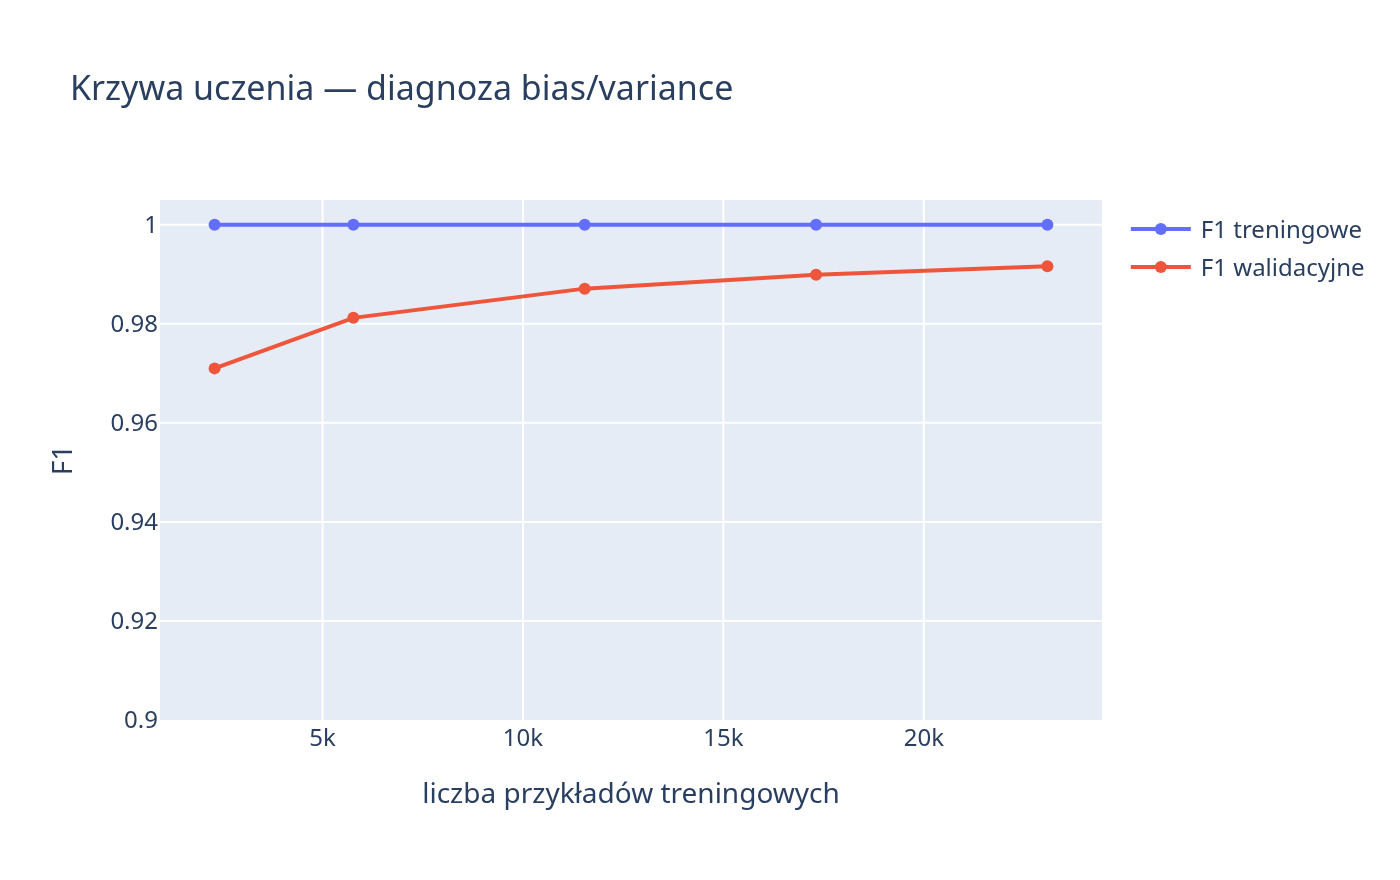
\includegraphics[width=0.72\textwidth]{figures/mlp_learning_curve.png}
  \caption{Krzywa uczenia. Obie krzywe wysoko i blisko siebie --- reżim
  niskiego biasu i niskiej wariancji przy suficie metryk zbioru.}
  \label{fig:lc}
\end{figure}

\subsection{Techniki regularyzacji}

Choć przeuczenie jest tu łagodne, model umożliwia jego kontrolę trzema technikami:
early stopping (zawsze aktywny), dropout i weight decay (L2). Tabela~\ref{tab:reg}
pokazuje wpływ na lukę train--val (miarę wariancji).

\begin{table}[H]
  \centering
  \caption{Wpływ regularyzacji na lukę train--val F1.}
  \label{tab:reg}
  \begin{tabular}{lccc}
    \toprule
    \textbf{Konfiguracja} & \textbf{F1 train} & \textbf{F1 val} & \textbf{luka} \\
    \midrule
    brak (dropout=0, wd=0) & 1{,}0000 & 0{,}9913 & 0{,}0087 \\
    dropout=0{,}3          & 1{,}0000 & 0{,}9916 & 0{,}0084 \\
    L2 (wd=$10^{-4}$)      & 0{,}9987 & 0{,}9939 & 0{,}0048 \\
    dropout=0{,}3 + L2     & 0{,}9987 & 0{,}9933 & 0{,}0054 \\
    \bottomrule
  \end{tabular}
\end{table}

Dropout i weight decay zmniejszają lukę (obniżają F1 treningowe, podtrzymując
walidacyjne), lecz F1 walidacyjne ledwie drga --- przy tak łatwym zbiorze
regularyzacja głównie kosmetyzuje lukę, a nie poprawia uogólnienia. Potwierdza to
diagnozę z krzywej uczenia.

\subsection{Interpretowalność cech}

Współczynniki regresji logistycznej (baseline) dają tanią, globalną wyjaśnialność
(Rys.~\ref{fig:cechy}). Stronę Real ciągną zwroty agencyjno-sprawozdawcze
(\texttt{said}, \texttt{on wednesday}, \texttt{president donald}), stronę Fake ---
zwroty potoczne/clickbaitowe (\texttt{via}, \texttt{read more}, \texttt{you},
\texttt{watch}, \texttt{video}). Co istotne, \emph{żaden} z usuniętych markerów
wycieku nie pojawia się na liście --- model uczy się stylu i tematu, a nie stempla
redakcyjnego.

\begin{figure}[H]
  \centering
  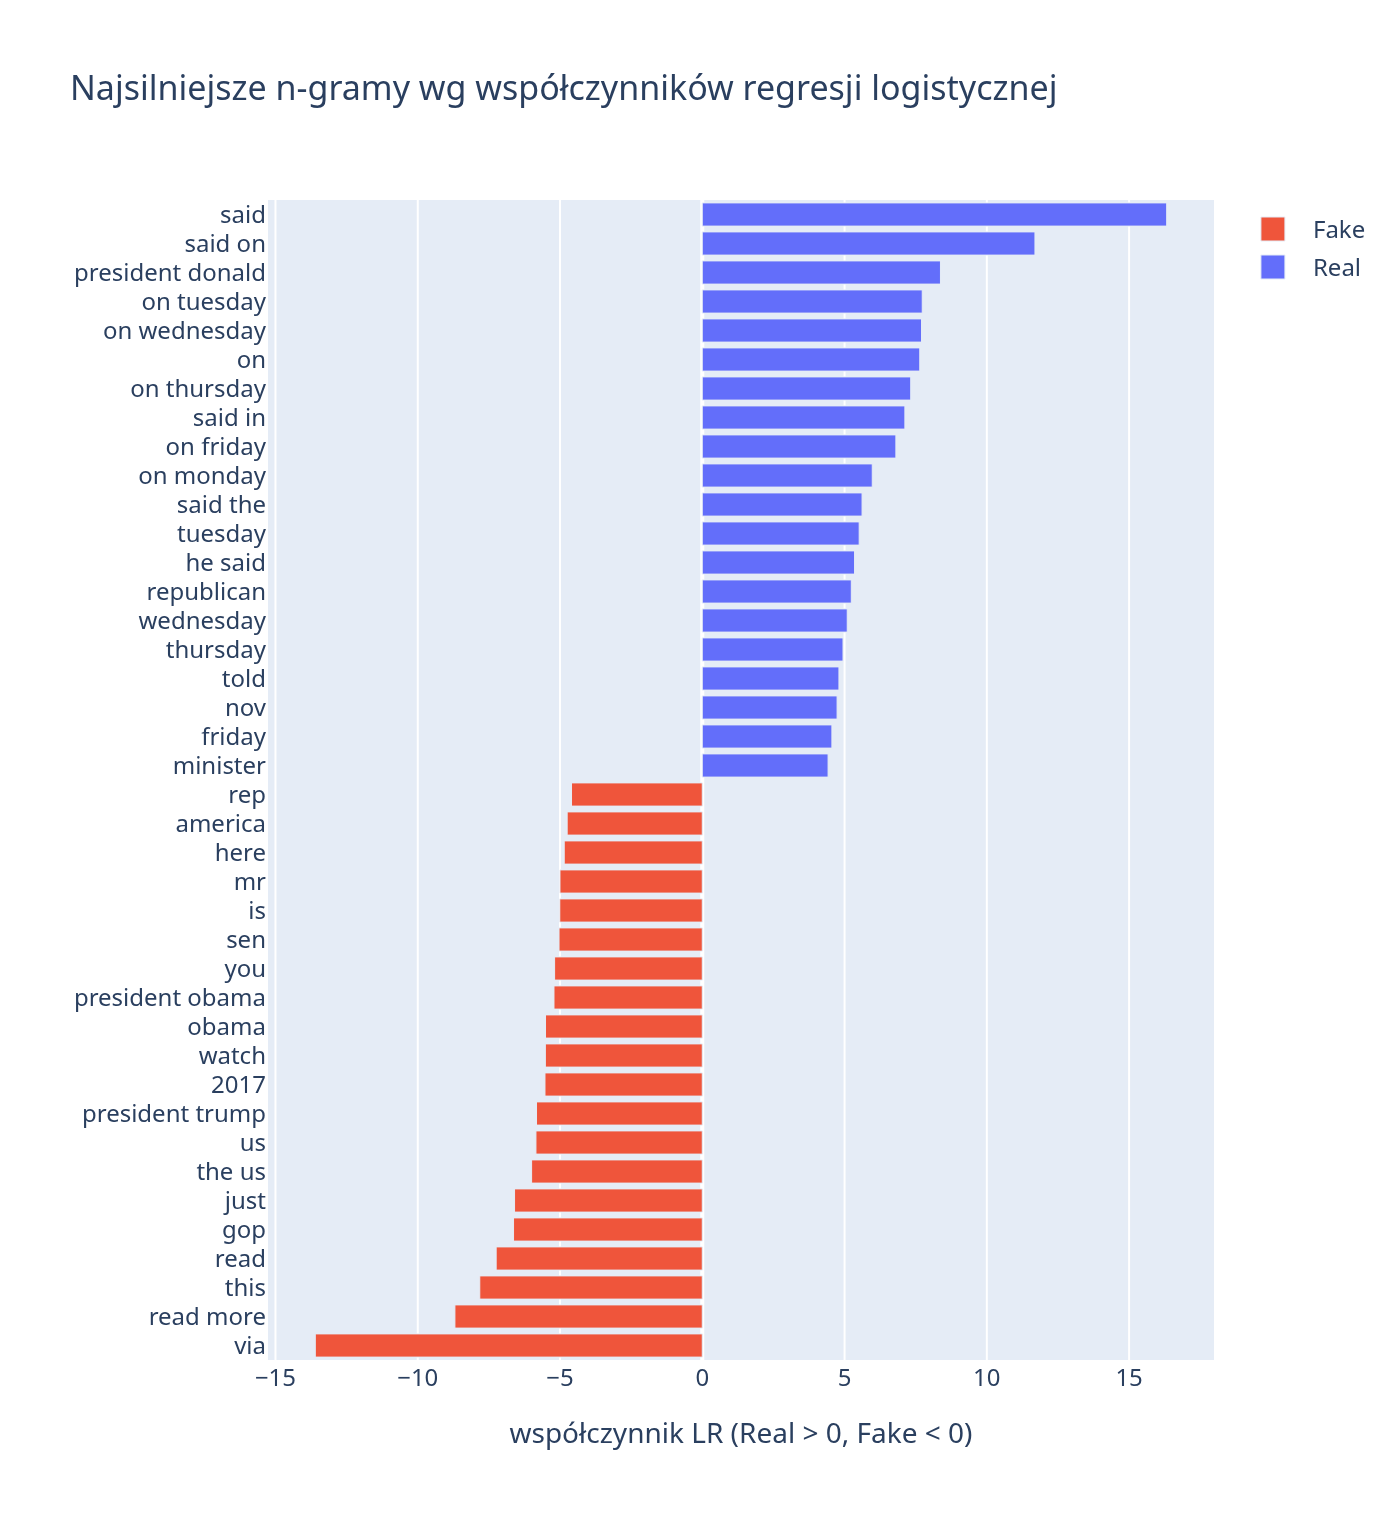
\includegraphics[width=0.85\textwidth]{figures/logreg_cechy.png}
  \caption{Najsilniejsze n-gramy wg współczynników regresji logistycznej
  (Real $> 0$, Fake $< 0$).}
  \label{fig:cechy}
\end{figure}
